%% Libs
\documentclass[polish,11pt,a4paper]{article}
\usepackage[a4paper, margin=2cm]{geometry}
\usepackage[T1]{fontenc}
\usepackage{babel}
\usepackage{graphicx}
\usepackage{ragged2e}
\usepackage{caption}
\usepackage{amsmath} 
\usepackage{amssymb} 
\usepackage{setspace}
\usepackage[utf8]{inputenc}
\usepackage{subfig}
\usepackage{cancel}
\usepackage{import}
\usepackage{svg}
\usepackage{pdfpages}
\usepackage{geometry}
%% start document
\begin{document}
%% Strona tytułowa
\setstretch{1.5}
\centering
\section*{WYDZIAŁ MECHANICZNY POLITECHNIKI BIAŁOSTOCKIEJ}
\section*{PROJEKT Z PRZEDMIOTU}
\section*{Systemy Autonomiczne}
\large
kod przedmiotu: MYAR2S22007M
\subsection*{Temat: Projektowanie układu sterowania i nawigacji
śmigłowca wielowirnikowego jako systemu
autonomicznego }
\vspace{2cm}
\raggedright
Autor: Ostaszewicz Dawid

Kierunek: Automatyka i Robotyka, II stopień

Specjalność: Informatyzacja Przemysłu

Semestr II

Prowadzący: dr inż. Leszek Ambroziak
\vspace{2cm}

Weryfikacja efektów uczenia się:

EK1: \dotso

EK2: \dotso

EK3: \dotso

EK4: \dotso

EK5: \dotso

EK6: \dotso

EK7: \dotso

EK8: \dotso

Uwagi prowadzącego:
\vspace{3cm}

ocena: \dotso
\clearpage

\justifying
\section*{Cel i zakres projektu}
Celem projektu jest zapoznanie się z systemami autonomicznymi na przykładzie śmigłowca
wielowirnikowego. Projekt obejmuje poznanie modelu śmigłowca, autonomi lotu oraz funkcji
i algorytmów niezbędnych do poprawnego planowania nakazanej linii drogi; generowaniem
drogi i sposobami aktywnej korelacji. 

\section*{Zadanie nr 1}
\subsection*{Treść}
Zapoznaj się z ukladem symulacyjnym śmigłowca czterowirnikowego; dostępnym
w bibliotece RMVT. Dodaj do układu symulacyjnego wyświetlanie parametrów lotu śmigłowca 
(porównaj wartości zadane parametrów nawigacyjnych z aktualnie mierzonymi). Zmodyfikuj
model dyniamiki śmigłowca zgodnie z parametrami zawartymi w tabeli. Sprawdź działanie układu
sterowania dla zmodyfikowanych parametrów modelu, popraw nastawy pętli regulacyjnych i sposób
stabilizacji śmigłowca. Poeksperymentuj z różnymi wzmocnieniami w układzie sterowania. Co się 
stanie jeśli zmniejszysz tłumienie lub zupełnie je usuniesz. Usuń kompensator siły grawitacji
i poeksperymentuj z dużą wartością wzmocnienia w układzie sterowania wysokością lub z innym 
typem regulatora.
\subsection*{Opracowanie}
Proces strojenia modelu rozpoczął się od wprawdzenia parametrów modelu w odpowiednie miejsce, co 
wprowadziło różnice między projektami. Dynamika śmigłowca zależy głównie od jego masy i danych tensora 
bezwładności. Żeby podjeść do strojenia regulatorów, na wejścia obiektów zostały podane sygnały skoku
jednostkowego.
\begin{figure}[ht]
    \centering
    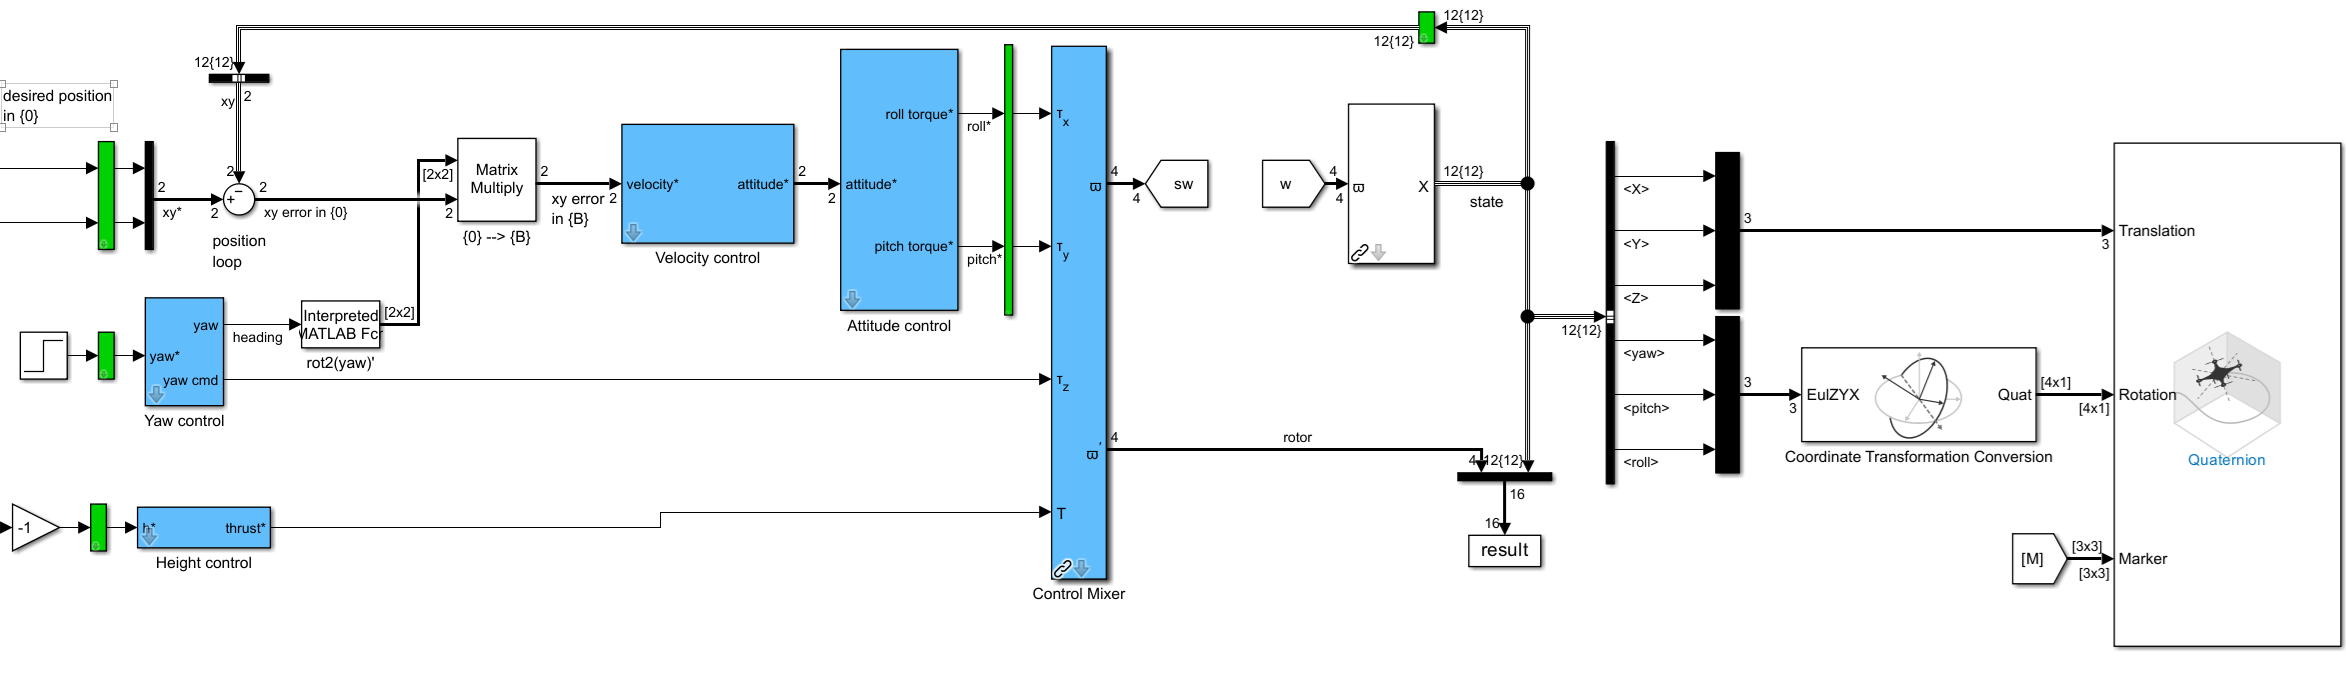
\includegraphics[width=1\linewidth]{strojenie/str-sch.png}
    \caption{Schemat obiektu}
    \label{fig:enter-label}
\end{figure}
Zgodnie z Rysunkiem 1, układ regulacji składa się z kaskadowo połączonych ukłdadów regulacji.
W takim wypadku strojenie powinno się rozpoczynać od wewnętrznych pętli, czyli "attitude control".
Układ regulacji zawiera pętle regulacji: położenia, prędkości, wysokości. Prędkość jest zależna od położenia
kątowego śmigłowca. Regulując położenie układ zadaje prędkości przez sterowanie kątami roll i pitch. Jak już 
zostało wspomniane najpierw były strojone regulatory znajdujące w najbardziej zagnieżdżonych pętlach, przemieszczając się 
od obszarów nadrzędnych układów regulacji automatycznej. Efektem działania powinna być trajektoria całkowicie aperiodyczna,
ponieważ jakiekolwiek przeregulowanie może być niebezpieczne dla śmigłowca. W procesie strojenia zostały uzyskane
odpowiedzi z Rysunku 2 i 3.
\begin{figure}[ht]
    \centering
    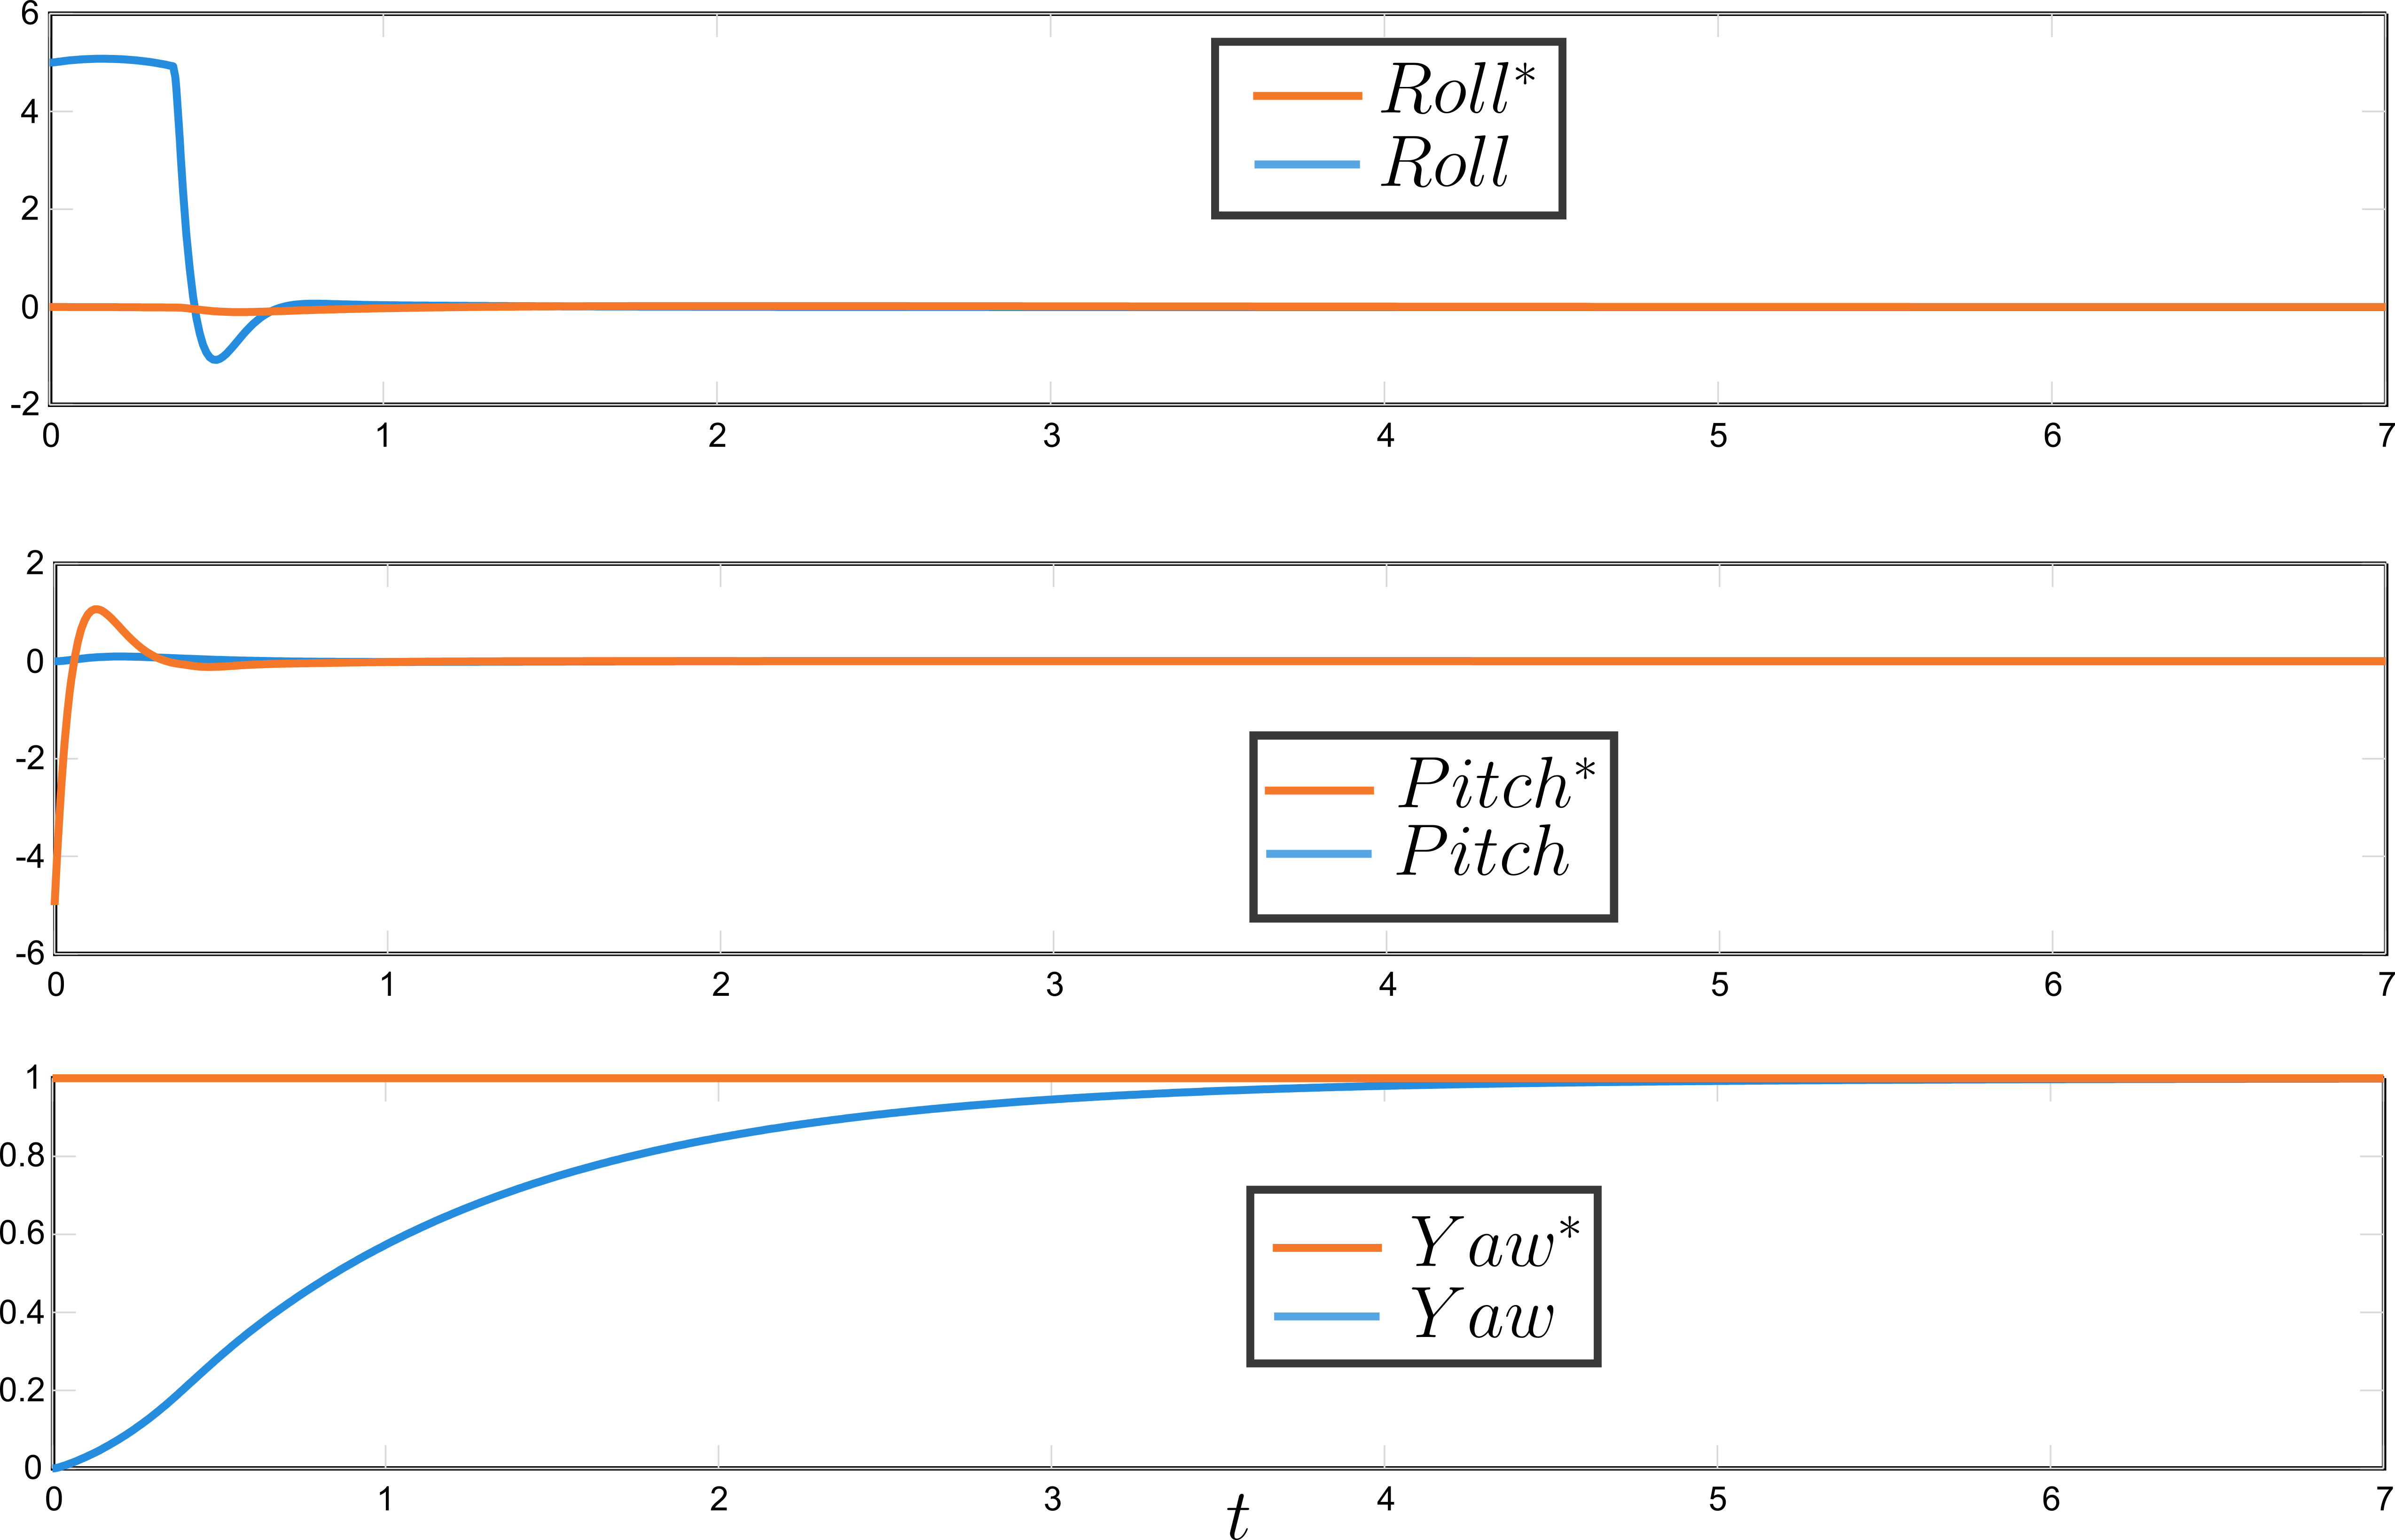
\includegraphics[width=0.7\linewidth]{strojenie/RLY.png}
    \caption{Odpowiedzi układu po strojeniu - XYZ}
    \label{fig:enter-label}
\end{figure}
\begin{figure}[ht]
    \centering
    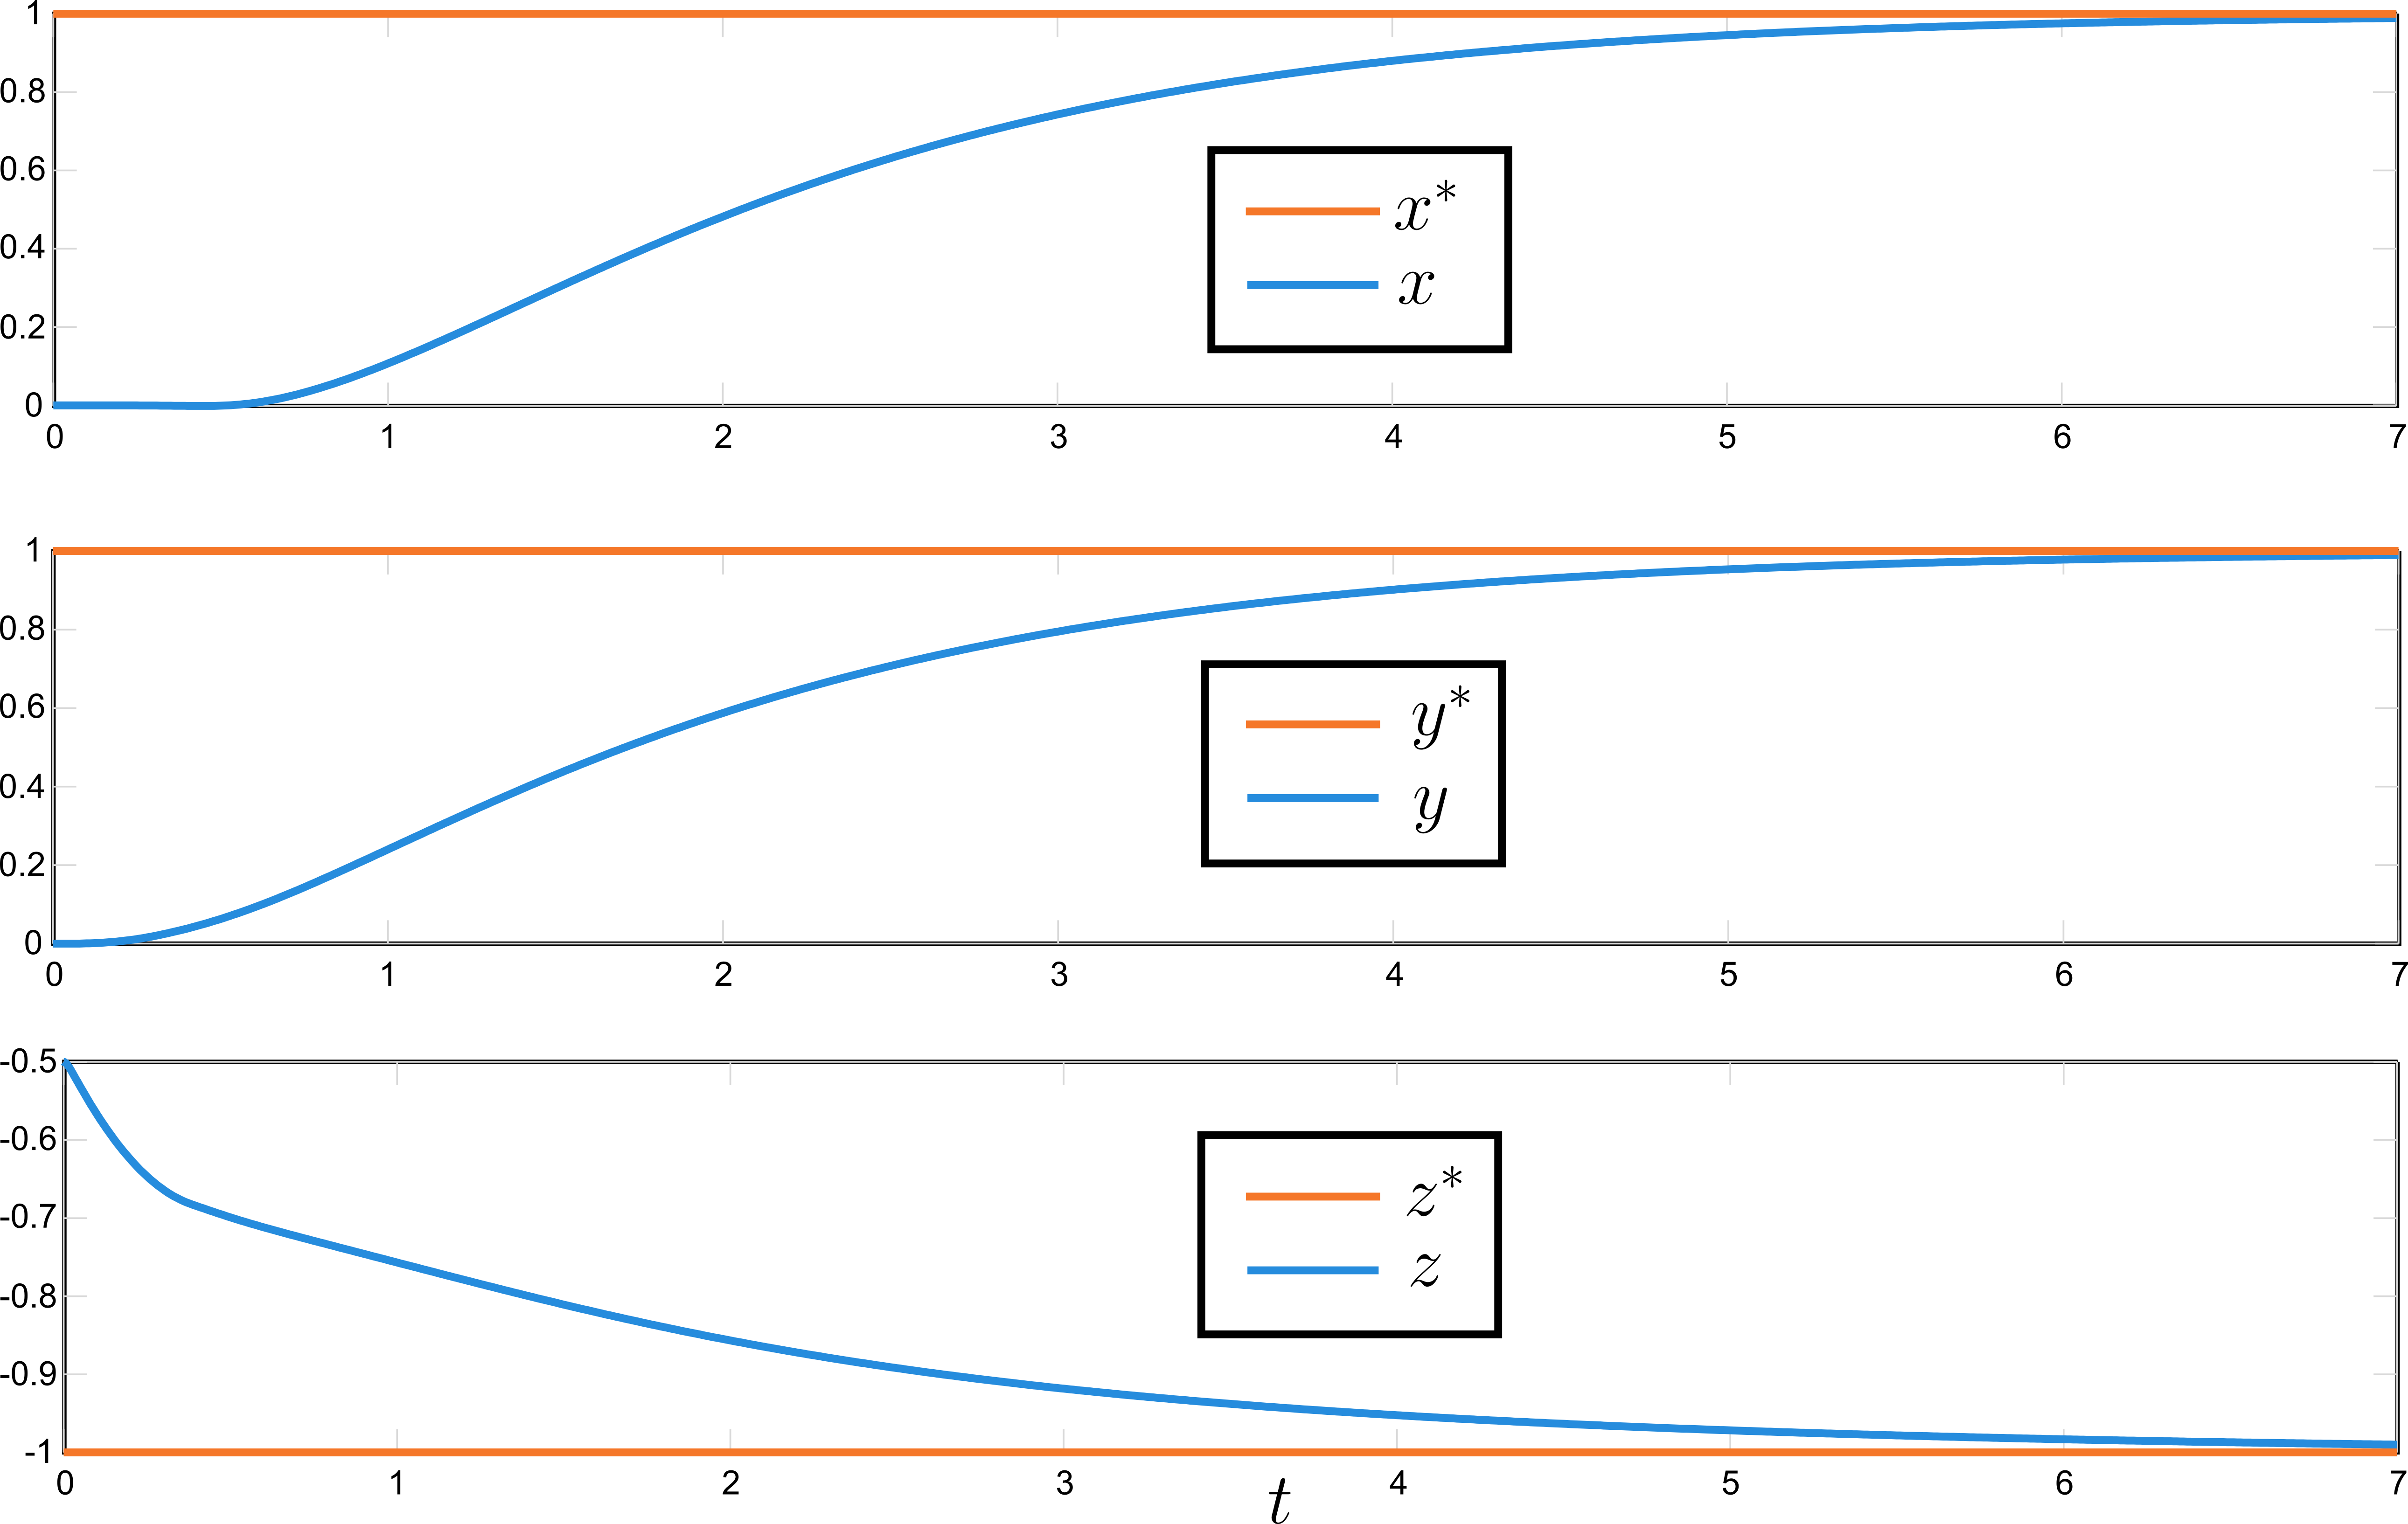
\includegraphics[width=0.7\linewidth]{strojenie/XYZ.png}
    \caption{Odpowiedzi układu po strojeniu - RLY}
    \label{fig:enter-label}
\end{figure}
Do układu regulacji wysokości kluczowe było odpowiednie ustawienie zmiennej "thrust feedforward", ponieważ 
układ powienien odpowiednio kompensować wpływ grawitacji. Nastawy regulatorów zostały zestawione w tabeli 1.
\begin{table}[h]
    \centering
    \caption{Nastawy}
    \label{tab:przyklad}
    \begin{tabular}{|c|c|c|c|}
        \hline
        Controller & P & D & Thrust feedforward \\ 
        \hline
        Attitude & 50 & 0.08 & - \\  
        \hline
        Velocity & 0.1 & 2 & - \\
        \hline 
        Yaw & 200 & 1 & - \\ 
        \hline
        Height & 500 & 2 & 58 \\  
        \hline
        Height & 5000 & 0.35 & 0 \\  
        \hline
    \end{tabular}
\end{table}

Jeśli chodzi o zmienną "thrust feedforward", można odpowiednio nastroić regulator wysokości bez niej, jednak wiąże się to z
efektami, które mogą nie być wygodne, lub możliwe do realizacji. Rysunek 4, przedstawia dziłanie nastaw dla regulatora
wysokości z zerową nastawą "Thrust feedforward" z tabeli 1.
\begin{figure}[ht]
    \centering
    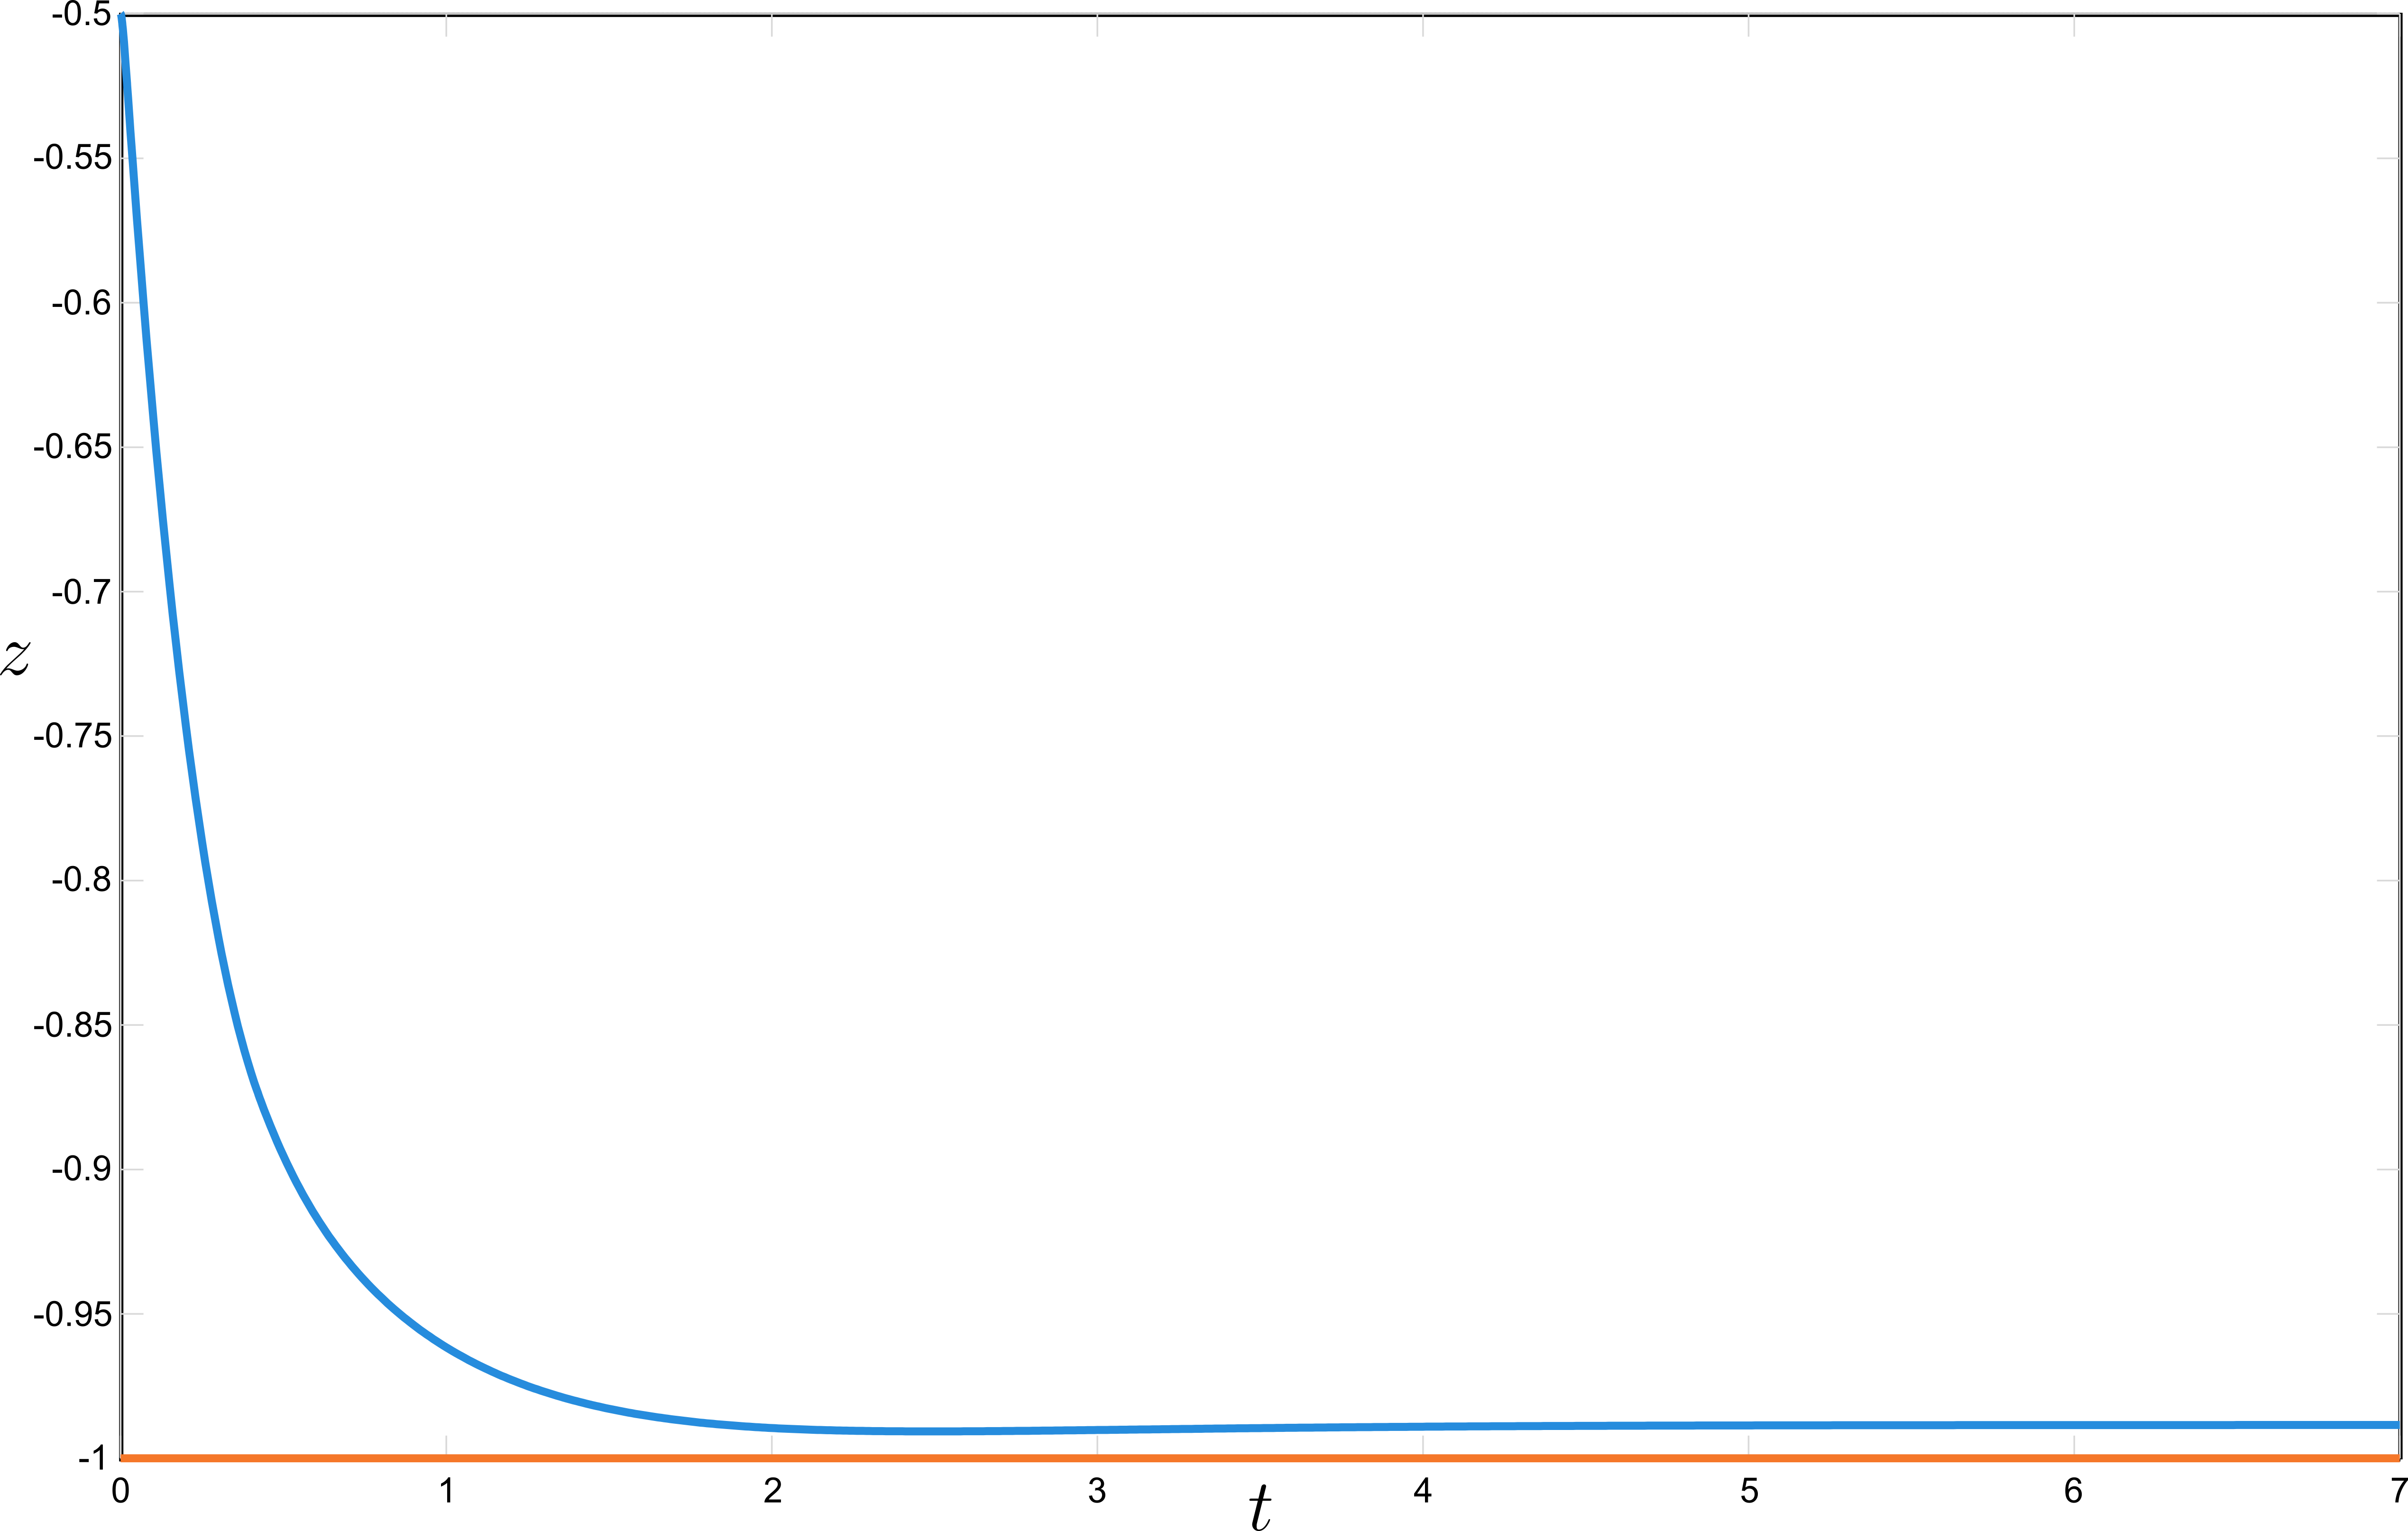
\includegraphics[width=0.7\linewidth]{strojenie/z.png}
    \caption{Odpowiedź układu dla strojenia bez kompensatora grawitacji}
    \label{fig:enter-label}
\end{figure}

Trzeba zauważyć, że przy takim strojeniu wielkości w torze sygnałów sterowania będą miały bardzo duże wartości
na wyjściach regulatorów, co w większości przypadków może nie być możliwe w realizacji. Poza tym układ posiada jeszcze
mały uchyb. 
\subsection*{Podsumowanie}
Strojenie regulatorów należy rozpoczynać od wewnętrznych pętli regulacji; przechodząć do nadrzędnych. Można nastroić regulator
wysokości bez kompensatora wysokości, jednak jego funkcjonowanie może okazać się niedogodne w realizacji praktycznej.
\section*{Zadanie nr 2}
\subsection*{Treść}
Opracuj funkcję realizującą ruch balistyczny śmigłowca. Niech quadrotor wystartuje
pod kątem 45 stopni do poziomu, następnie wyzeruj cały ciąg. Sprawdź uzyskaną trajektorię śmigłowca.
Spróbuj opracować funkcję realizującą lot balistyczny do zadanego punktu na powierzchni.

\subsection*{Opracowanie}
Istnieje wiele podejść do problemu realizacji ruchu balistycznego śmigłowca wielowirnikowego.
Pierwszą z nich jest sterowanie śmigłowcem do określonego punktu przestrzeni; żeby następnie, jeszcze 
w trakcie przyspieszenia wyłączyć lub ograniczyć ciąg. W efekcie takiego zabiegu trajektoria powinna być
zbliżona do balistycznej. Poprzednie rozwiązanie jest problematyczne pod względem uchwycenia chwili, 
posiadania przyspieszenia. Jeśli ciąg wyłączy się zbyt późno, przyspieszenie obiektu w osiach XY może być
zbyt małe, żeby utworzyć dobrą trajektorię balistyczną. Prostrzym podejściem będzie zadawanie pozycji
liniowo narastającej w czasie. W wyniku pracy z regulatorami o pojedyńczym całkowaniu, śmigłowiec, co prawda
nie będzie nadążał za wartością zadaną; będzie posiadał stały uchyb, co jest wadą zastosowanych regulatorów o 
jednokrotnym całkowaniu, jednak w każdym razie obiekt w określonej sytuacji powinien posiadać stałe przyspieszenie.
Jeśli ciąg zostanie ograniczony, obiekt będzie się zniżał. Trajektoria będzie zbliżona 
do balistycznej. Rysunek 5 przedstawia schemat Simulinka do realizowanego zadania.

\begin{figure}[ht]
    \centering
    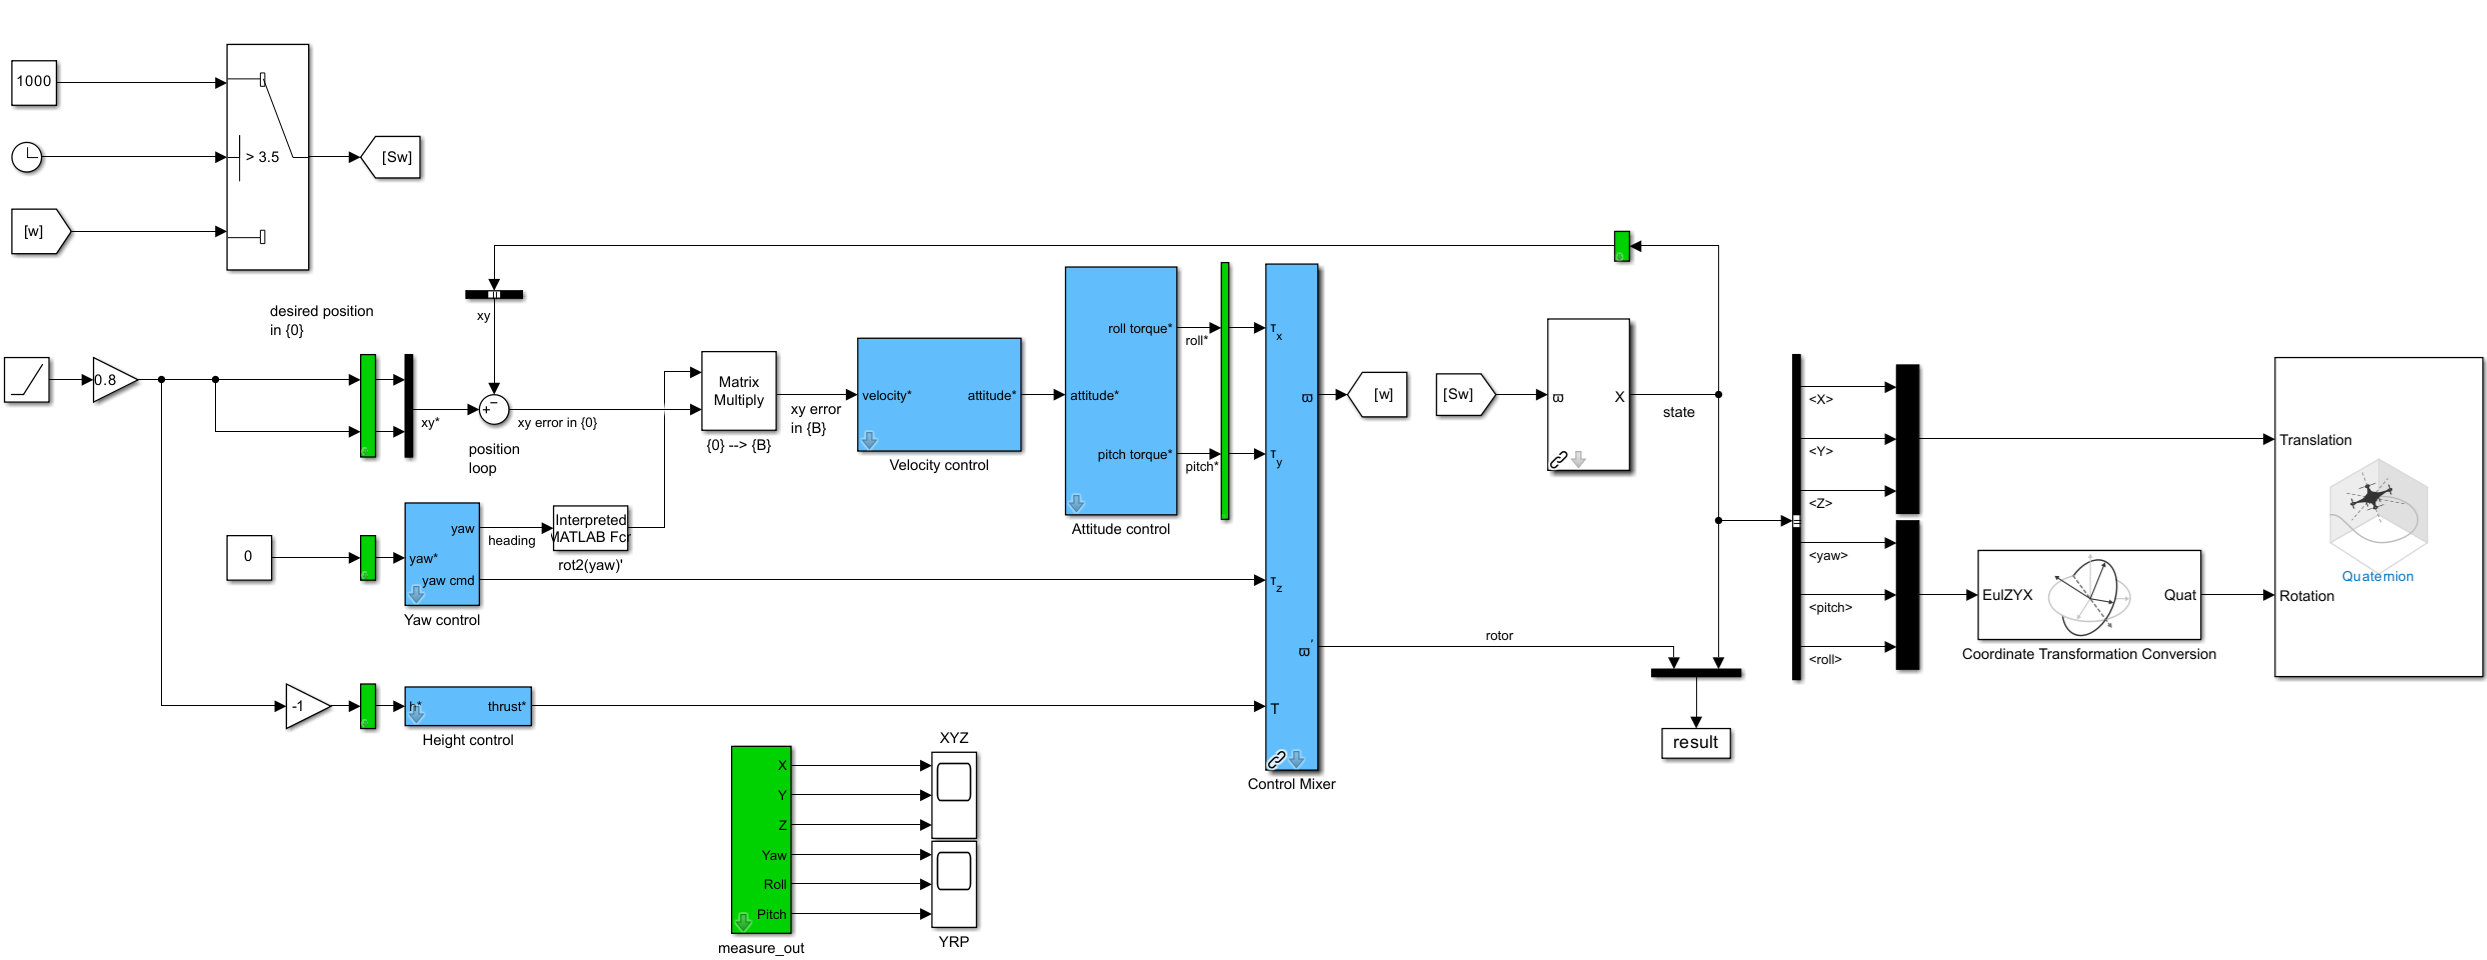
\includegraphics[width=1\linewidth]{paraboliczna/sc_parab.png}
    \caption{Schemat realizacji trajektorii balistycznej}
    \label{fig:enter-label}
\end{figure}

Ciąg generowany przez śmigła będzie ograniczany, w różnych odstępach czasu. Badanie odległości punktu
lądowania od czasów wyłączenia, umożliwi wyprowadzenie zależności czasu ograniczenia ciągu od odległości;
ostatecznie taki zabieg umożliwi stworzenie realacji, która pozwoli zadawać punkt lądowania, Rysunek ...
Znając realcję czasu wyłączenia od odległości na jakiej ląduje dron (można obliczyć z eq...).
\begin{equation}
    s = \sqrt{x^{2}+y^{2}}
\end{equation}
Można z pomocą Rysunku 7 aproksymować odległość punktu lądowania. W takim kontekście zadanie punktu lądowania powinno odpowiadać
wektorowi przemieszczenia w płaszczyźnie XY i relacji czasu ograniczenia ciągu. Pierwszą rzeczą będzie zadanie określenia kąta wektora przemieszczenia
w płaszczyźnie XY, eq (2,3)


\begin{equation}
    k_{x} = \sin \arctan \frac{x^{*}}{y^{*}}
\end{equation}

\begin{equation}
    k_{y} = \cos \arctan \frac{x^{*}}{y^{*}}
\end{equation}
Natomiast moduł wektora przemieszczenia określa równanie aproksymacji drogi eq (4))

\begin{equation}
    t = \sqrt{x^{2}+y^{2}} - 0.13
\end{equation}

\begin{figure}[ht]
    \centering
    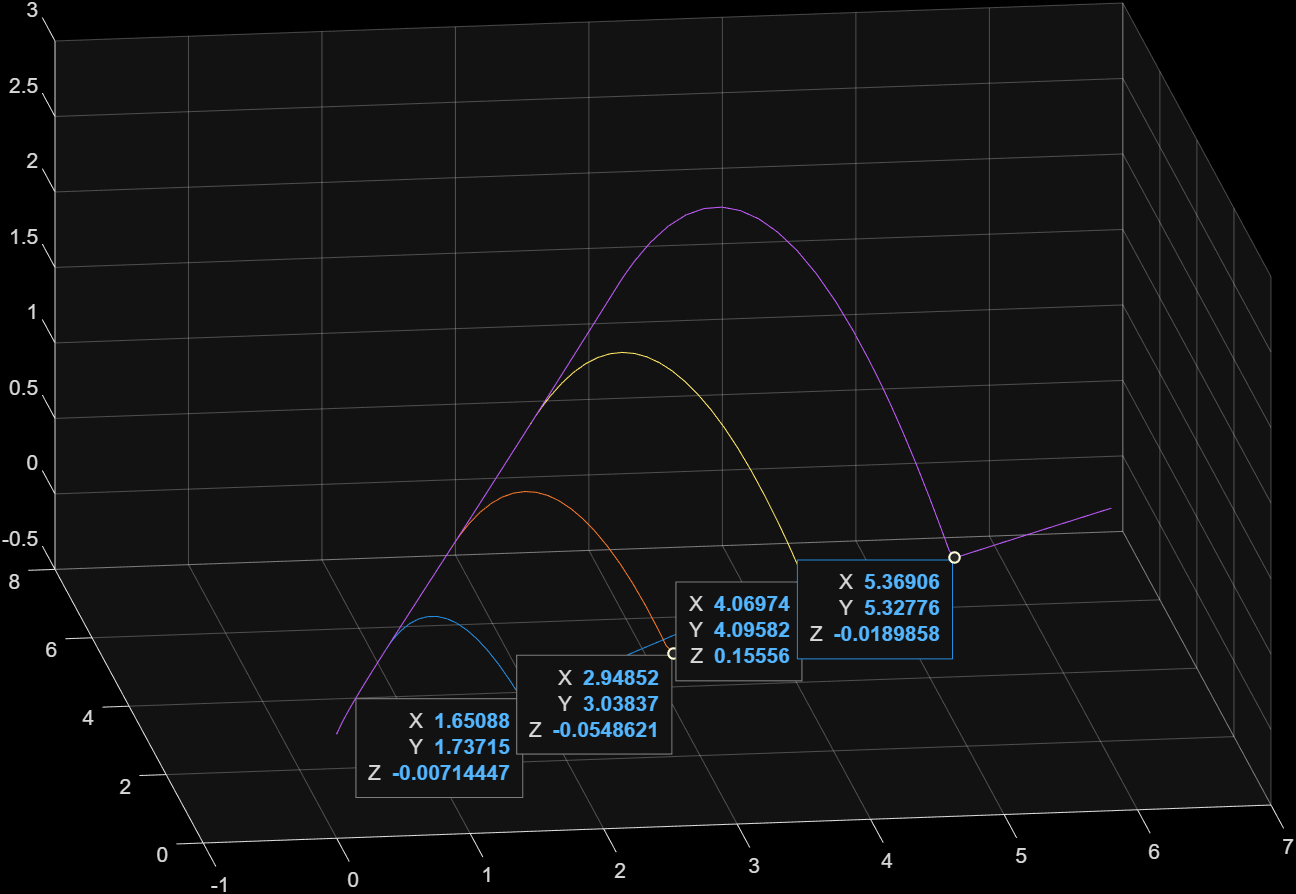
\includegraphics[width=0.65\linewidth]{paraboliczna/parabole.png}
    \caption{Otrzymane trajektorie balistyczne}
    \label{fig:enter-label}
\end{figure}

\begin{figure}[h]
    \centering
    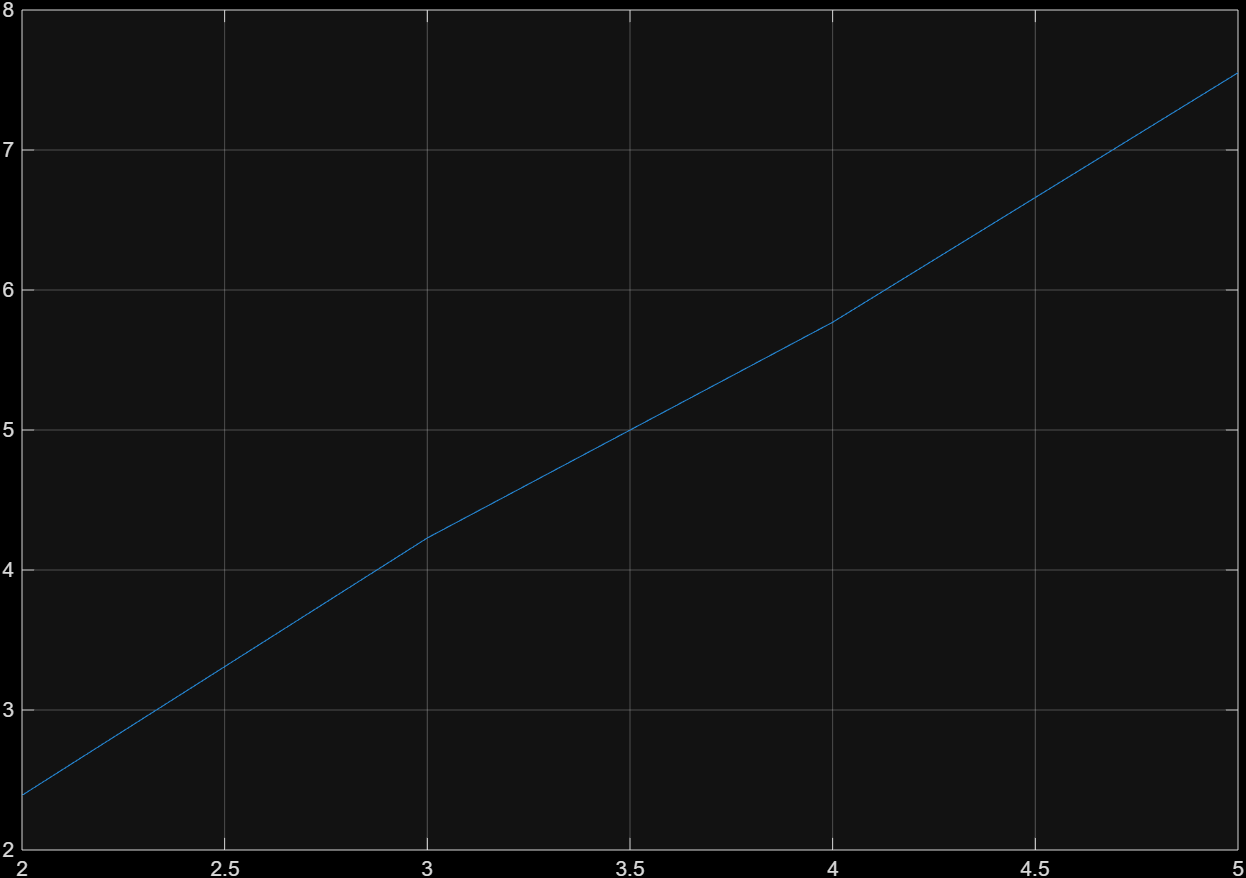
\includegraphics[width=0.65\linewidth]{paraboliczna/st.png}
    \caption{Odległość od punktu startowego}
    \label{fig:enter-label}
\end{figure}

\break
\subsection*{Wnioski}
Wykonane badania pozwalają określić, zależności na wykonanie balistycznego lotu śmigłowca wielowirnikowego.
Zastosowanie liniowo narastających wartości zadanych umożliwia zadanie stałego przyspieszenia obiektu, natomiast
ograniczenie ciągu wymusza ruch po trajektorii balistycznej. Wykonane badanie wraz z aproksymacją umożliwia 
wyprowadzenie równań na lot balistyczny w przybliżeniu do punktu zadanego.

\section*{Zadanie nr 3}
\subsection*{Treść}
Opracuj funkcję realizującą automatyczne lądowanie śmigłowca w oparciu o dostępne 
sygnały pomiarowe (lądowanie może być aktywowane w dowolnym momencie, ze wskazaniem miejsca laowania,
po aktywowaniu funkcji automatycznego lądowania śmigłowiec przerywa wcześniej realizowany scenariusz,
podąża do punktu lądowania, przechodzi do zawisu, po czym łagodnie ląduje)

\subsection*{Opracowanie}
Pierwszą fazą lądowania jest przerwanie czynności, które obecnie są realizowane przez drona. Wartości
zadane w osiach x i y będą zapamiętywane przy użyciu bloku z Rysunku 8

\begin{figure}[ht]
    \centering
    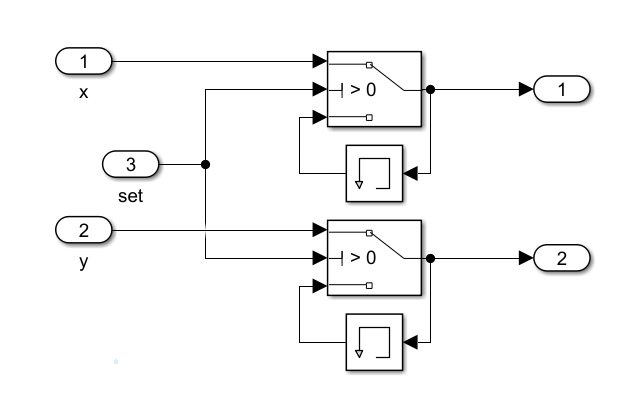
\includegraphics[width=1\linewidth]{lądowanie/set.png}
    \caption{Funkcja pamięci stanu trajektorii w płaszczyźnie xy}
    \label{fig:enter-label}

\end{figure}

Funkcja zadaje zapamiętane wartości, a dron je utrzymuje. W tej fazie również będzie dochodziło
do zniżania pułapu lotu, do wartości około 30 cm przy użyciu przełącznika. Założenie drugiej fazy
lądowania: jeśli dron osiągnie pułap mniejszy niż 35 cm, zacznie stopniowo ograniczać ciąg silników. Natomiast
w trzeciej fazie; po osiągnięciu 20 cm silniki zostają wyłączone, żeby ograniczyć turbulencje związane z
oddziaływaniem podłoża. Wnętrze bloku automatycznego lądowania zestawia Rysunek 9

\begin{figure}[ht]
    \centering
    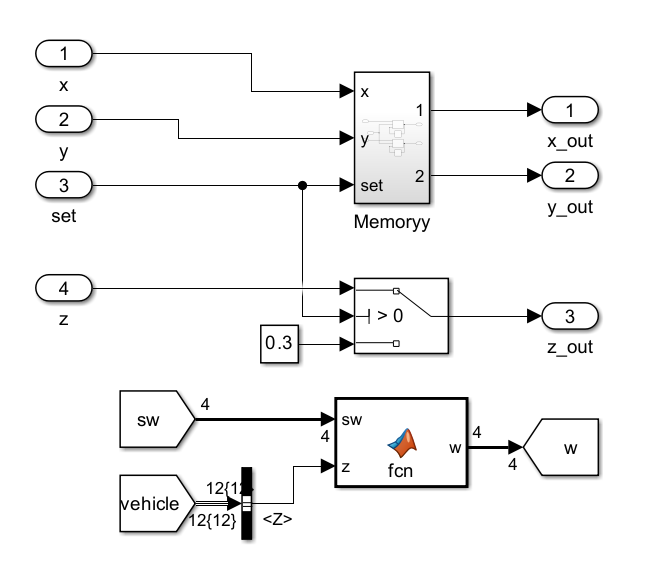
\includegraphics[width=0.65\linewidth]{lądowanie/lond.png}
    \caption{Automatyczne lądowanie - blok}
    \label{fig:enter-label}

\end{figure}

Wejście set jest związane z działaniem przycisku. W trakcie lotu można przełączyć przełącznik, który rozpocznie
sekwencję automatycznego lądowania. Wnętrze bloku matlab function:

\begin{verbatim}
    function w = fcn(sw,z)

    if (z > -0.35) && (z < -0.30)
        w = 0.8*sw;
    elseif (z >= -0.30) && (z < -0.20)
        w = 0.6*sw;
    elseif (z >= -0.20)
        w = 0.1*sw;
    else
        w = sw;
    end
\end{verbatim}
\break
\begin{figure}[h]
    \centering
    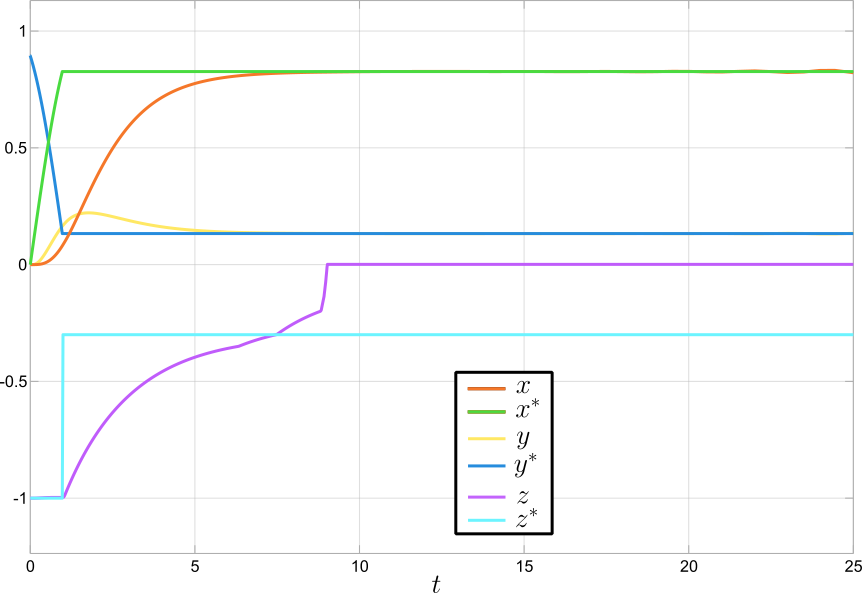
\includegraphics[width=0.65\linewidth]{lądowanie/land.png}
    \caption{Automatyczne lądowanie - sygnały}
    \label{fig:enter-label}

\end{figure}

\break
\subsection*{Podsumowanie}
Po czasie około sekundy przełącznik automatycznego lądowania został włączony, zmienił wartość wejścia "set" bloku automatycznego
lądowania. Następnie zadane trajektorie zostały wstrzymane na jednym punkcie w płaszczyźnie xy; następowało 
zniżenie pułapu lotu, następnie układ przechodzi do fazy kaskadowego wyłączania ciągu silników i przechodzi
do sekwencji wielopoziomowego lądowania. W ostatniej fazie silniki są wyłączane i dron ląduje na ziemi.

\section*{Zadanie nr 4}
\subsection*{Treść}
Opracuj algorytm realizujący lot śmigłowca czterowirnikowego po zadanych punktach drogi.
Zadane punkty powinny być definiowane przed rozpoczęciem lotu i przechowywane w 
macierzy. Dodatkowo powinny być zaznaczone na wizualizacji lotu śmigłowca.
\subsection*{Opracowanie}
Rysunek 11 przedstawia schemat realizacji lotu śmigłowca po nakazanych punktach drogi.

\begin{figure}[ht]
    \centering
    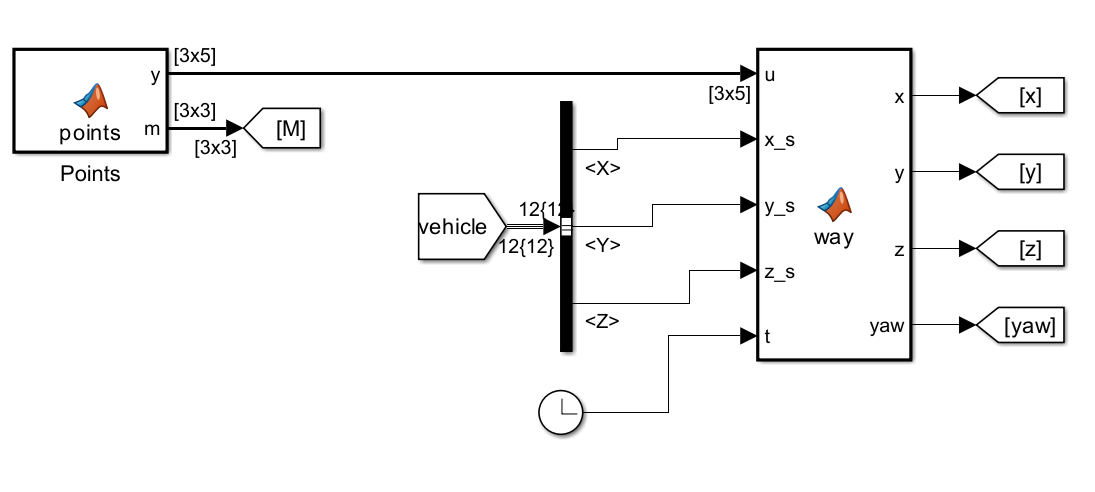
\includegraphics[width=1\linewidth]{nakazane/nakaz-sch.png}
    \caption{Schemat algorytmu śledzenia waypointów}
    \label{fig:enter-label}

\end{figure}

Funkcja "points" przechowuje macierz współrzędnych kolejnych punktów, wraz z kątem yaw, który 
ma osiągnąć dron podczas lotu do nakazanego punktu oraz czas jaki dron ma przebywać w nakazanej sferze
drogi. 

\begin{verbatim}
    function [y, m] = points()
persistent P T;

if isempty(P)
    % ---- x --- y --- z --- yaw --- time----
    P = [  1,    1,    1,     1,      0.5; ...
           2,    1,    3,     0.5,    0.5; ...
          -1,    2,    2,    -0.5,    0.5];
end

if isempty(T)
    T = [  1,    1,    -1; ...
           2,    1,    -3; ...
           -1,   2,    -2];
end

y = P;
m = T;
\end{verbatim}

Wartości są przypisywane do odpowiednich indeksów zgodnie z opisem zawartym w funkcji. Macierz T
przechowuje współrzędne punktow, które są potrzebne do ich wyświetlania na wizualizacji UAV. 

Funkcja "way" realizuje algorytm śledzenia waypointów.

\begin{verbatim}
    function [x, y, z, yaw] = way(u, x_s, y_s, z_s, t)

persistent i
persistent start_time

if isempty(i)
    i = 1;
end

if isempty(start_time)
    start_time = t;
end

       
        x = u(i, 1);
        y = u(i, 2);
        z = u(i, 3);
        yaw = u(i, 4);
        w_time = u(i,5);

        distance = sqrt((x - x_s)^2 + (y - y_s)^2 + (z + z_s)^2);
        disp(sprintf('Distance: %.3f', distance))
        if distance < 0.1
            elapsed_time = t - start_time;
            disp(sprintf('Start time: %.3f', start_time))
            disp(sprintf('Elapsed time: %.3f', elapsed_time))
            if elapsed_time >= w_time
                i = i+1;
                if i >= height(u)
                    i  = height(u);
                end
                disp("waypoint")

            end
        else
            start_time = t;
        end
   
end
\end{verbatim}

Funkcja przyjmuje argumenty, które są niezbędne do wykonanania algorytmu. Na początku definiowana jest
zmienna i, która przyjmuje wartość początkową równa jeden. Następnie układ zadaje współrzędne i kąt, yaw; jaki
ma osiągnąć dron dolatując do punktu drogi; jako pierwszy rząd macierzy. Później podczas próbkowania symulacji
na bieżąco obliczany jest dystans do obecnie zadanego waypointu. Jeśli wayipoint nie został osiągnięty
czas start\_time jest stale aktualizowany. 
\begin{figure}[ht]
    \centering
    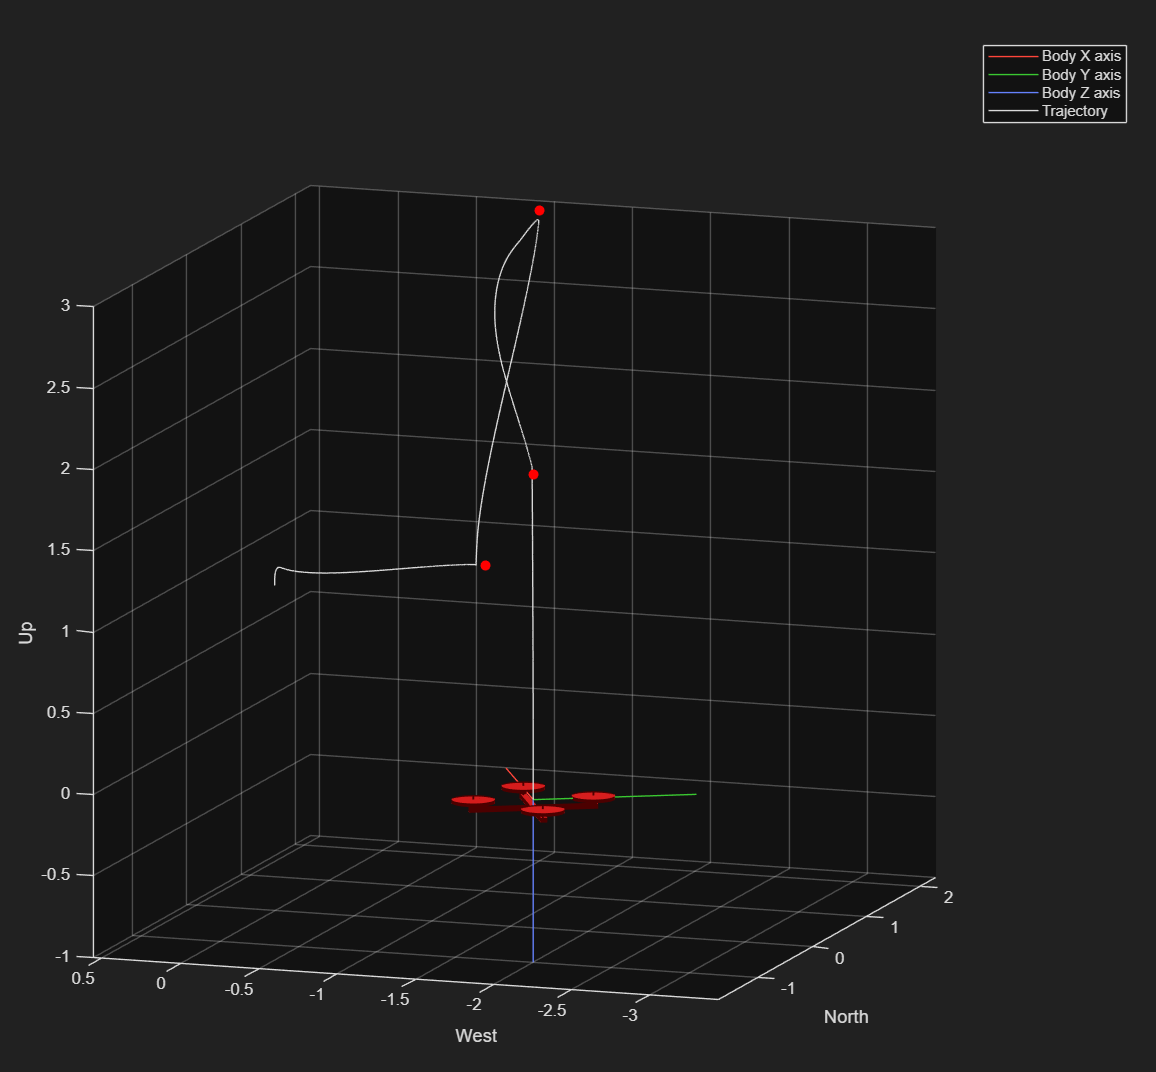
\includegraphics[width=0.7\linewidth]{nakazane/nakaz.png}
    \caption{Śledzenie waypointów}
    \label{fig:enter-label}

\end{figure}
Po przekroczeniu waypointu start\_time nie jest zmieniany i oblicza się czas
od wejścia w sferę nakazanego punktu drogi. Jeśli czas przebywania w waypoincie zadany w tablicy zostanie osiągnięty
zmienna i pzechodzi do następnej iteracji w tablicy i tak, aż do wykonania wszystkich zdanych punktów. Żeby nie wychodzić poza 
zakres tablicy z nakazanymi punktami dorgi jest ustawione ograniczenie, które sprawia, że jeśli zakres zostanie przekroczony 
zmienna i przybiera wartość ostatniego elementu. Po wykonaniu całej drogi można np. przełączyć przycisk i rozpocząć
sekwencję automatycznego lądowania; Rysunek 12.
\section*{Podsumowanie projektu}
Zaprojektowany algorytm, który umożliwia zadawanie śmigłowcowi punktów drogi,
 otwiera możliwości implementacji i dalszego rozwoju środowiska. Przykładowo,
  można zastosować algorytmy planowania trasy do generowania macierzy zadanych
   punktów. W trakcie realizacji projektu można także zwrócić uwagę na niezbędne czujniki,
    które są kluczowe w takich aplikacjach. Aby dron mógł poprawnie realizować zadane 
    algorytmy, konieczne są m.in. czujniki GPS, kamery oraz IMU, często w konfiguracjach
     redundantnych i komplementarnych. Fundamentem sterowania systemami
      autonomicznymi jest dostęp do pokładowych przyrządów pomiarowych, które zapewniają 
      dokładność wymaganą dla danego zastosowania.

Moduł automatycznego lądowania wymaga praktycznej weryfikacji, gdyż symulowanie
 zjawisk, takich jak turbulencje spowodowane przez reakcję podłoża, jest trudne.
  Ze względu na ten problem konieczne jest dostrojenie algorytmu lądowania do warunków
   środowiska, szczególnie w zakresie odpowiedniego sterowania ciągiem silników na różnych
    wysokościach i fazach lądowania, by precyzyjnie określić moment ich wyłączenia.

Ogólnie rzecz biorąc, projekt został opracowany w środowisku pozbawionym wpływu
 warunków zewnętrznych, co znacznie ułatwiło jego realizację. W warunkach rzeczywistych,
  np. przy określonym poziomie wiatru i zakłóceniach czujników, dostosowanie regulatorów
   byłoby bardziej wymagające. W praktycznych zastosowaniach korzystne mogłoby okazać się 
   wdrożenie zaawansowanych algorytmów regulacji, aby minimalizować wpływ zakłóceń na działanie 
   układu sterowania.
\clearpage
   \newgeometry{paper=a3paper, landscape}
   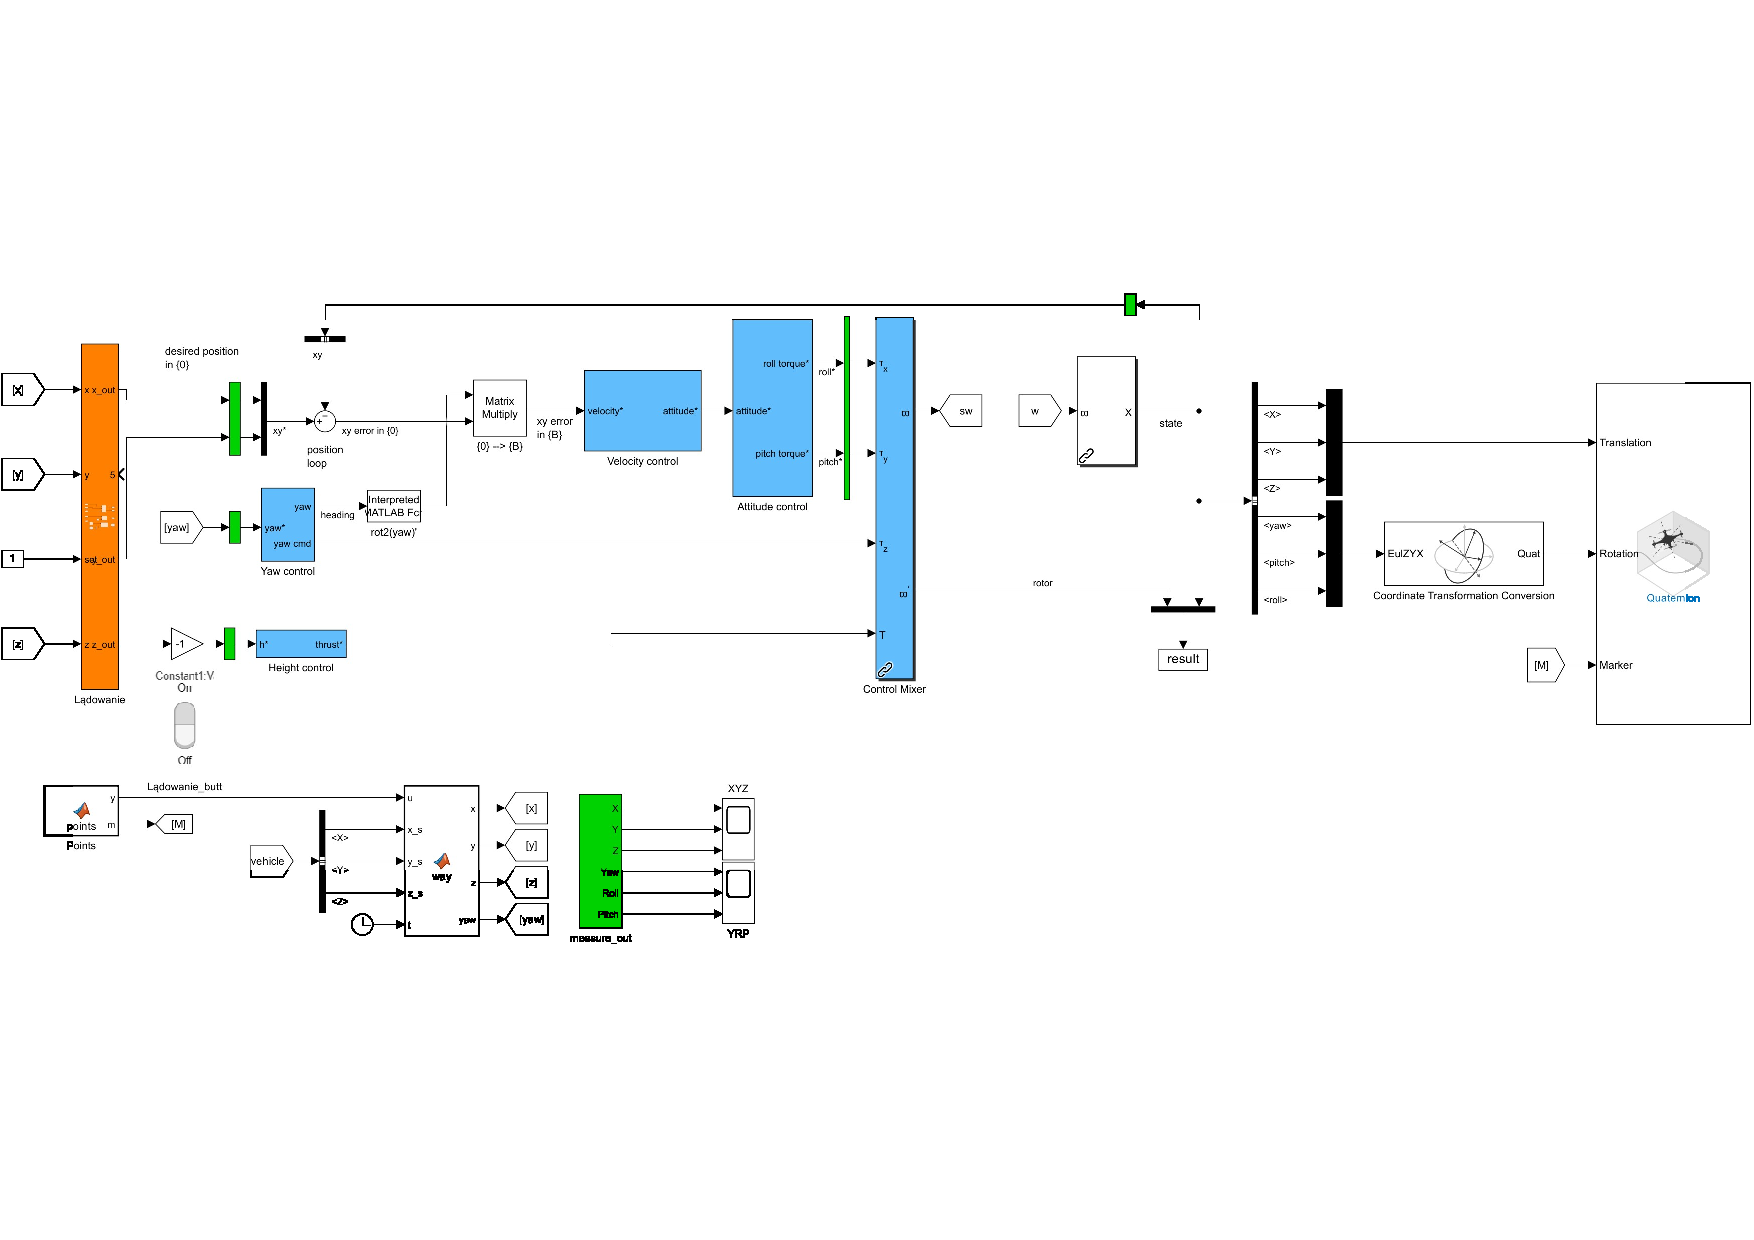
\includepdf[pages=1-6, angle=90]{schematy.pdf}
\end{document}